\section{\large Исследовательская часть}
\label{cha:research}

В данном разделе будут приведены примеры работы разработанной программы и проведён анализ времени выполнения запросов с использованием: чистого SQL, ORM (Object-Relational Mapping) и Query Builder. Результаты иссследования позволят точнее определять основные требования к базе данных при её выборе для проектирования системы, тем самым облегчая процесс выбора наиболее подходящей для конкретной задачи СУБД.	

%\subsection{Результаты разработки}

\subsection{Постановка исследования}

Целью исследование является сравнение времени обработки запроса, выполненного при помощи чистого SQL, ORM и Query Builder. Для запросов, выполненных при помощи ORM и Query Builder необходимо дополнительно сравнить время, в течение которого выполняются SQL запросы.

Иссследование было проведенно с замером времени выполнения запроса, возвращающего список всех пациентов. Замеры времени были осущствлены 500 раз (изолированных друг от друга) для увеличения точности. Было учтено кэширование буфера (очищен кэш перед проведением замеров), а также учтено влияние прогрева буферного кэша на результаты замеров (не учитывался первый запрос, во время которого происходит прогрев кэша).

Технические характеристики устройства, на котором выполнялось тестирование:

\begin{itemize}[label=---]
	\item Операционная система: macOS Ventura 13.2.1 (22D68) \cite{macos};
	\item Память: 16 Гб с тактовой частотой 2133 МГц LPDDR3 \cite{memory};
	\item Процессор: Intel Core™ i7-8559U \cite{intel} с тактовой частотой  2.70 ГГц;
	\item Видеокарта: Intel Iris Plus Graphics 655 \cite{graphics} c объёмом памяти 1536 Мб.
\end{itemize}

Тестирование проводилось на ноутбуке, включенном в сеть электропитания. Во время тестирования ноутбук был нагружен только системой тестирования (работающим приложением) и системным окружением операционной системы.

\subsection{Сравнение времени обработки}

Результаты измерений  времени обработки запросов. выполненных при помощи чистого SQL, ORM и Query Builder, показаны на рисунке \ref{fig:research}.

\begin{figure}[h]
	\centering
	\captionsetup{justification=centering}
	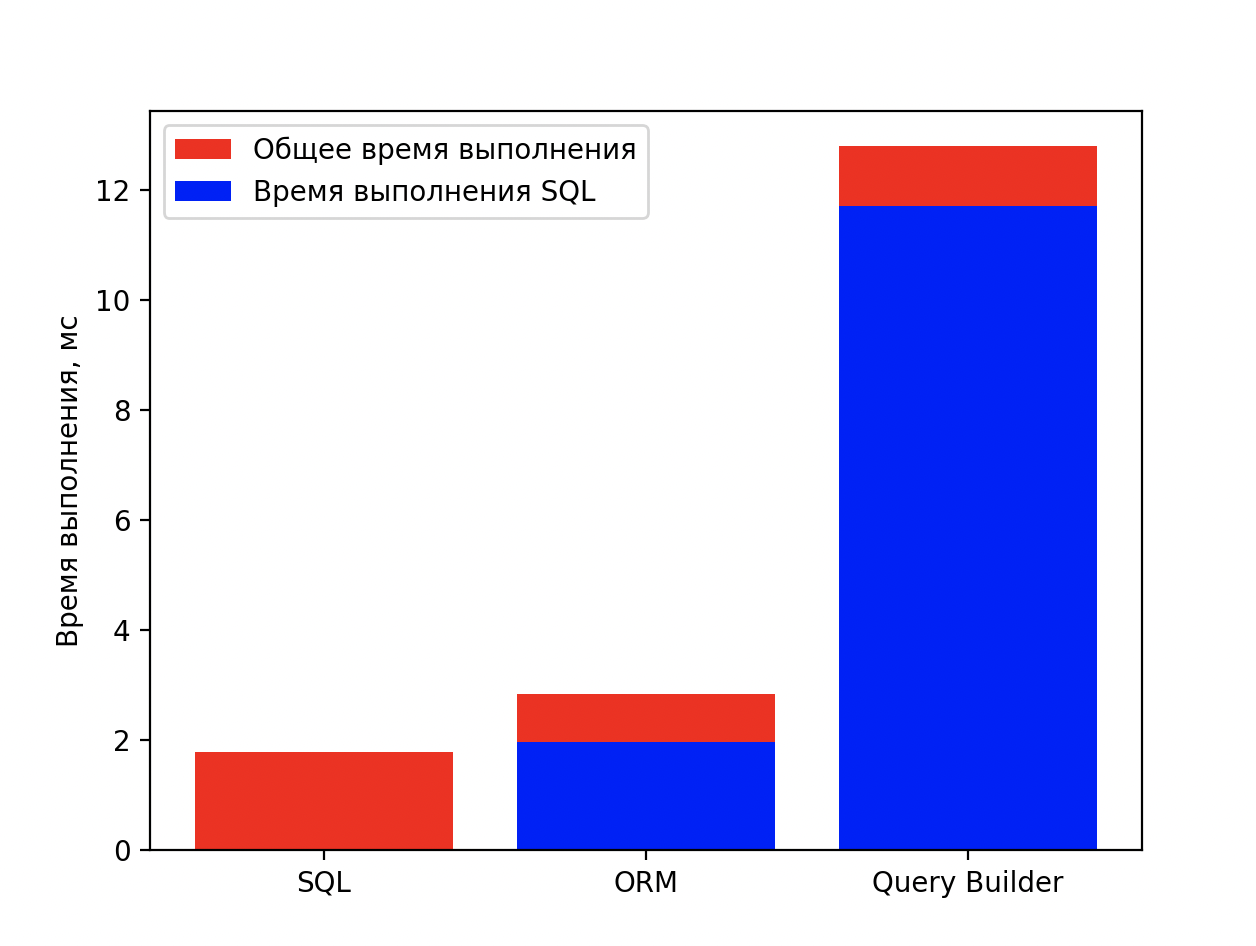
\includegraphics[width=130mm]{img/research.png}
	\caption{Результаты замеров времени обработки запросов}
	\label{fig:research}
\end{figure}


Исходя из полученных результатов, выполнение запросов при помощи чистого SQL является наиболее быстрым способом (1.78 миллисекунды). Использование ORM является более эффективным, чем применение Query Builder (2.84 миллисекунды для ORM и 12.79 миллисекунды для Query Builder). При использовании ORM лишь 1.96 миллисекунды было затрачено на выполнение SQL, что лишь немного превышает время обработки запроса при помощи чистого SQL (разница составила 0.18 мс для ORM против 9.93 мс для Query Builder).

\subsection*{Вывод}
В данном разделе были описаны элементы интерфейса и приведены примеры работы разработанной программы. 
Графический интерфейс предоставляет возможность просмотреть список методов реализовнного API и их подробные характеристики (тип метода, адрес, используемые структуры), а также отправить конкретный запрос, осуществив ввод необходимых аргументов.
Проведён анализ времени обработки запросов с использованием чистого SQL, ORM и Query Builder, из результатов следует, что использование чистого SQL является самым быстрым способом (1.78 мс), однако не намного превосходит время, затраченное на выполнение SQL при использовании ORM (на 0.18 мс). Использование Query Builder занимает больше всего времени (12.79 мс).




